%!TEX root = ../../thesis.tex

\section{\sys{CoQA}: A Conversational QA Challenge}
\label{sec:coqa-dataset}

In this section, we introduce \sys{CoQA}, a novel dataset for building \tf{Co}nversational \tf{Q}uestion \tf{A}nswering systems. We develop \sys{CoQA} with three main goals in mind. The first concerns the nature of questions in a human conversation. As an example seen in Figure~\ref{fig:coqa-example}, in this conversation, every question after the first is dependent on the conversation history. At present, there are no large scale reading comprehension datasets which contain questions that depend on a conversation history and this is what \sys{CoQA} is mainly developed for.\footnote{Concurrent with our work, \newcite{choi2018quac} also created a conversational dataset with a similar goal, but it differs in many key design decisions. We will discuss it in Section~\ref{sec:coqa-future}.}

The second goal of \sys{CoQA} is to ensure the naturalness of answers in a conversation. As we discussed in the earlier chapters, most existing reading comprehension datasets either restrict answers to a contiguous span in a given passage, or allow free-form answers with a low human agreement (e.g., \sys{NarrativeQA}). Our desiderata are 1) the answers should not be only span-based so that anything can be asked and the conversation can flow naturally. For example, there is no extractive answer for $Q_4$ \ti{How many?} in Figure~\ref{fig:coqa-example}. 2) It still supports reliable automatic evaluation with a a strong human performance. Therefore, we propose that the answers can be free-form text (abstractive answers), while the extractive spans act as rationales for the actual answers. Therefore, the answer for $Q_4$ is simply \ti{Three} while its rationale is spanned across multiple sentences.

The third goal of \sys{CoQA} is to enable building QA systems that perform robustly across domains. The current reading comprehension datasets mainly focus on a single domain which makes it hard to test the generalization ability of existing models. Hence we collect our dataset from seven different domains --- children's stories, literature, middle and high school English exams, news, Wikipedia, science articles and Reddit. The last two are used for out-of-domain evaluation.

\subsection{Task Definition}
\label{sec:coqa-task}

\begin{figure}[!t]
\begin{tabular}{p{\columnwidth}}
\toprule
The Virginia governor's race, billed as the marquee battle of an otherwise anticlimactic 2013 election cycle, is shaping up to be a foregone conclusion. Democrat Terry McAuliffe, the longtime political fixer and moneyman, hasn't trailed in a poll since May. Barring a political miracle, Republican Ken Cuccinelli will be delivering a concession speech on Tuesday evening in Richmond. In recent ...\\
\\
$Q_1$:               What are the candidates {\bf \color{magenta} running} for?\\
$A_1$:               Governor\\
$R_1$: The Virginia governor's race\\
\vspace{0em}
$Q_2$:               {\bf \color{magenta} Where}?\\
$A_2$:               Virginia \\
$R_2$: The Virginia governor's race\\
\vspace{0em}
$Q_3$:               Who is the democratic candidate?\\
\vspace{-0.6em}{\bf \color{blue} A$_3$}:               {\bf \color{orange} Terry McAuliffe} \\
$R_3$: Democrat Terry McAuliffe\\
\vspace{0em}
$Q_4$:               Who is {\bf \color{orange} his} opponent?\\
\vspace{-0.6em}{\bf \color{blue} A$_4$}:               {\bf \color{red} Ken Cuccinelli} \\
$R_4$ Republican Ken Cuccinelli\\
\vspace{0em}
$Q_5$:               What party does {\bf \color{red} he} belong to?\\
$A_5$:               Republican \\
$R_5$: Republican Ken Cuccinelli\\
\vspace{0em}
$Q_6$:               Which of {\bf \color{blue} them} is winning?\\
$A_6$:               Terry McAuliffe \\
$R_6$: Democrat Terry McAuliffe, the longtime political fixer and moneyman, hasn't trailed in a poll since May\\
\bottomrule
\end{tabular}
\longcaption{Another example in \sys{CoQA} with entity of focus changes}{\label{fig:coqa-example2}A conversation showing coreference chains in colors. The entity of focus changes in $Q_4$, $Q_5$, $Q_6$.}
\end{figure}

We first define the task formally. Given a passage $P$, a conversation consists of $n$ turns, and each turn consists of $(Q_i, A_i, R_i), i = 1, \ldots n$, where $Q_i$ and $A_i$ denote the question and the answer in the $i$-th turn, and $R_i$ is the rationale which supports the answer $A_i$ and must be a single span of the passage. The task is defined as to answer the next question $Q_i$ given the conversation so far: $Q_1, A_1, \ldots, Q_{i -1}, A_{i - 1}$. It is worth noting that we collect $R_i$ with the hope that they can help understand how answers are derived and improve training our models, while \ti{they are not provided during evaluation}.

For the example in Figure~\ref{fig:coqa-example2}, the conversation begins with question $Q_1$. We answer $Q_1$ with $A_1$ based on the evidence $R_1$ from the passage. In this example, the answerer wrote only the \ti{Governor} as the answer but selected a longer rationale \ti{The Virginia governor's race}. When we come to $Q_2$ \ti{Where?}, we must refer back to the conversation history since otherwise its answer could be \ti{Virginia} or \ti{Richmond} or something else. In our task, conversation history is indispensable for answering many questions. We use conversation history $Q_1$ and $A_1$ to answer $Q_2$ with $A_2$ based on the evidence $R_2$.  For an unanswerable question, we give \ti{unknown} as the final answer and do not highlight any rationale.

In this example, we observe that the entity of focus changes as the conversation progresses. The questioner uses \ti{his} to refer to \ti{Terry} in $Q_4$ and \ti{he} to \ti{Ken} in $Q_5$. If these are not resolved correctly, we end up with incorrect answers. The conversational nature of questions requires us to reason from multiple sentences (the current question and the previous questions or answers, and sentences from the passage). It is common that a single question may require a rationale spanned across multiple sentences (e.g., $Q_1$ $Q_4$ and $Q_5$ in Figure~\ref{fig:coqa-example}). We describe additional question and answer types in \ref{sec:coqa-data-analysis}.


\subsection{Dataset Collection}
We detail our dataset collection process as follows. For each conversation, we employ two annotators, a questioner and an answerer. This setup has several advantages over using a single annotator to act both as a questioner and an answerer:
1) when two annotators chat about a passage, their dialogue flow is natural compared to chatting with oneself; 2) when one annotator responds with a vague question or an incorrect answer, the other can raise a flag which we use to identify bad workers; and 3) the two annotators can discuss guidelines (through a separate chat window) when they have disagreements. These measures help to prevent spam and to obtain high agreement data.\footnote{Due to AMT terms of service, we allowed a single worker to act both as a questioner and an answerer after a minute of waiting. This constitutes around 12\% of the data.}

\begin{figure}[!t]
  \center
  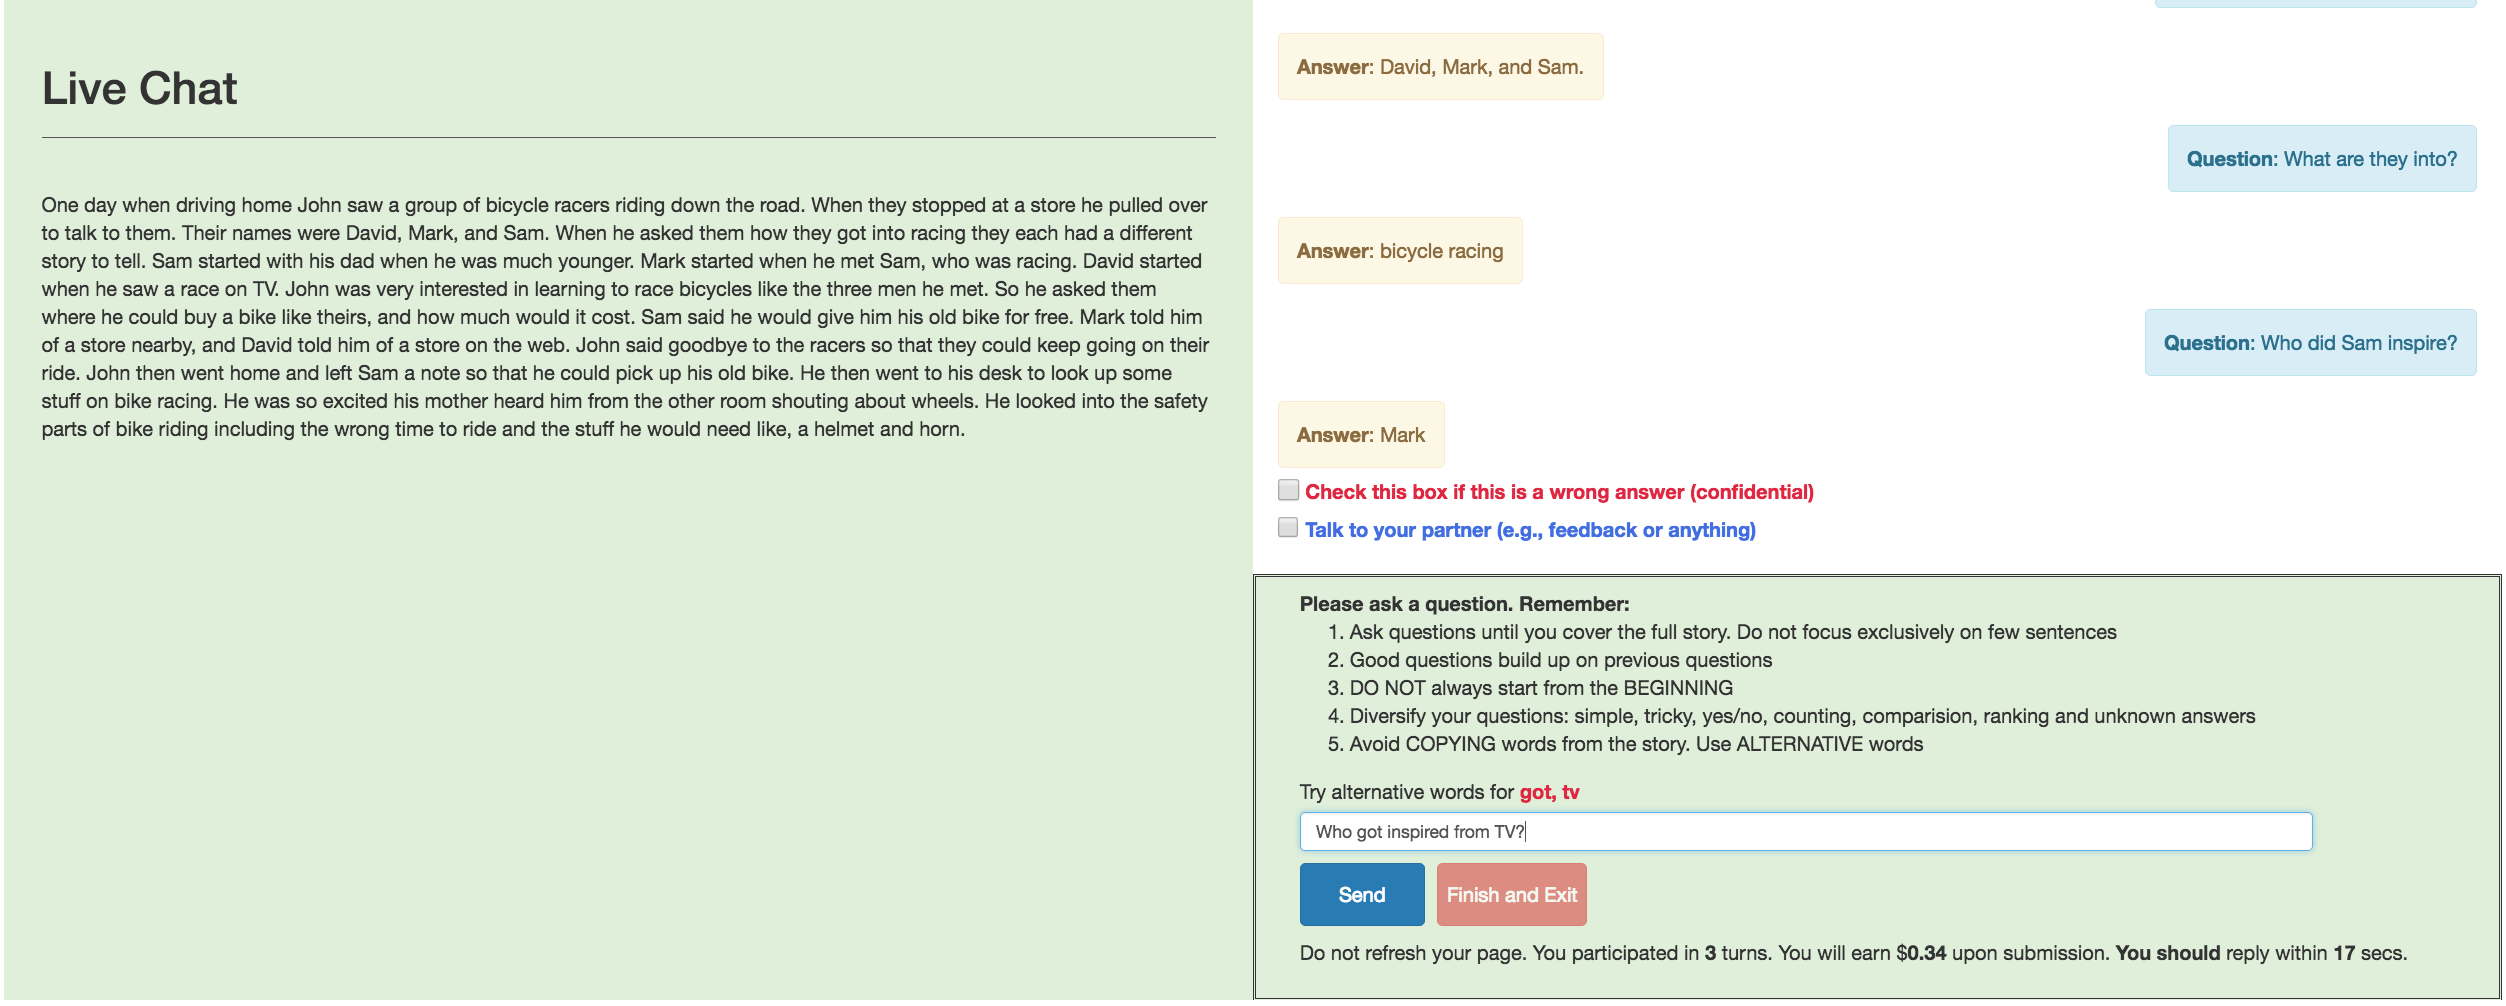
\includegraphics[scale=0.18]{img/coqa_questioner.png}
  \longcaption{The questioner interface of \sys{CoQA}}{\label{fig:coqa-questioner}The questioner interface of our \sys{CoQA} dataset.}
\end{figure}

\begin{figure}[!t]
  \center
  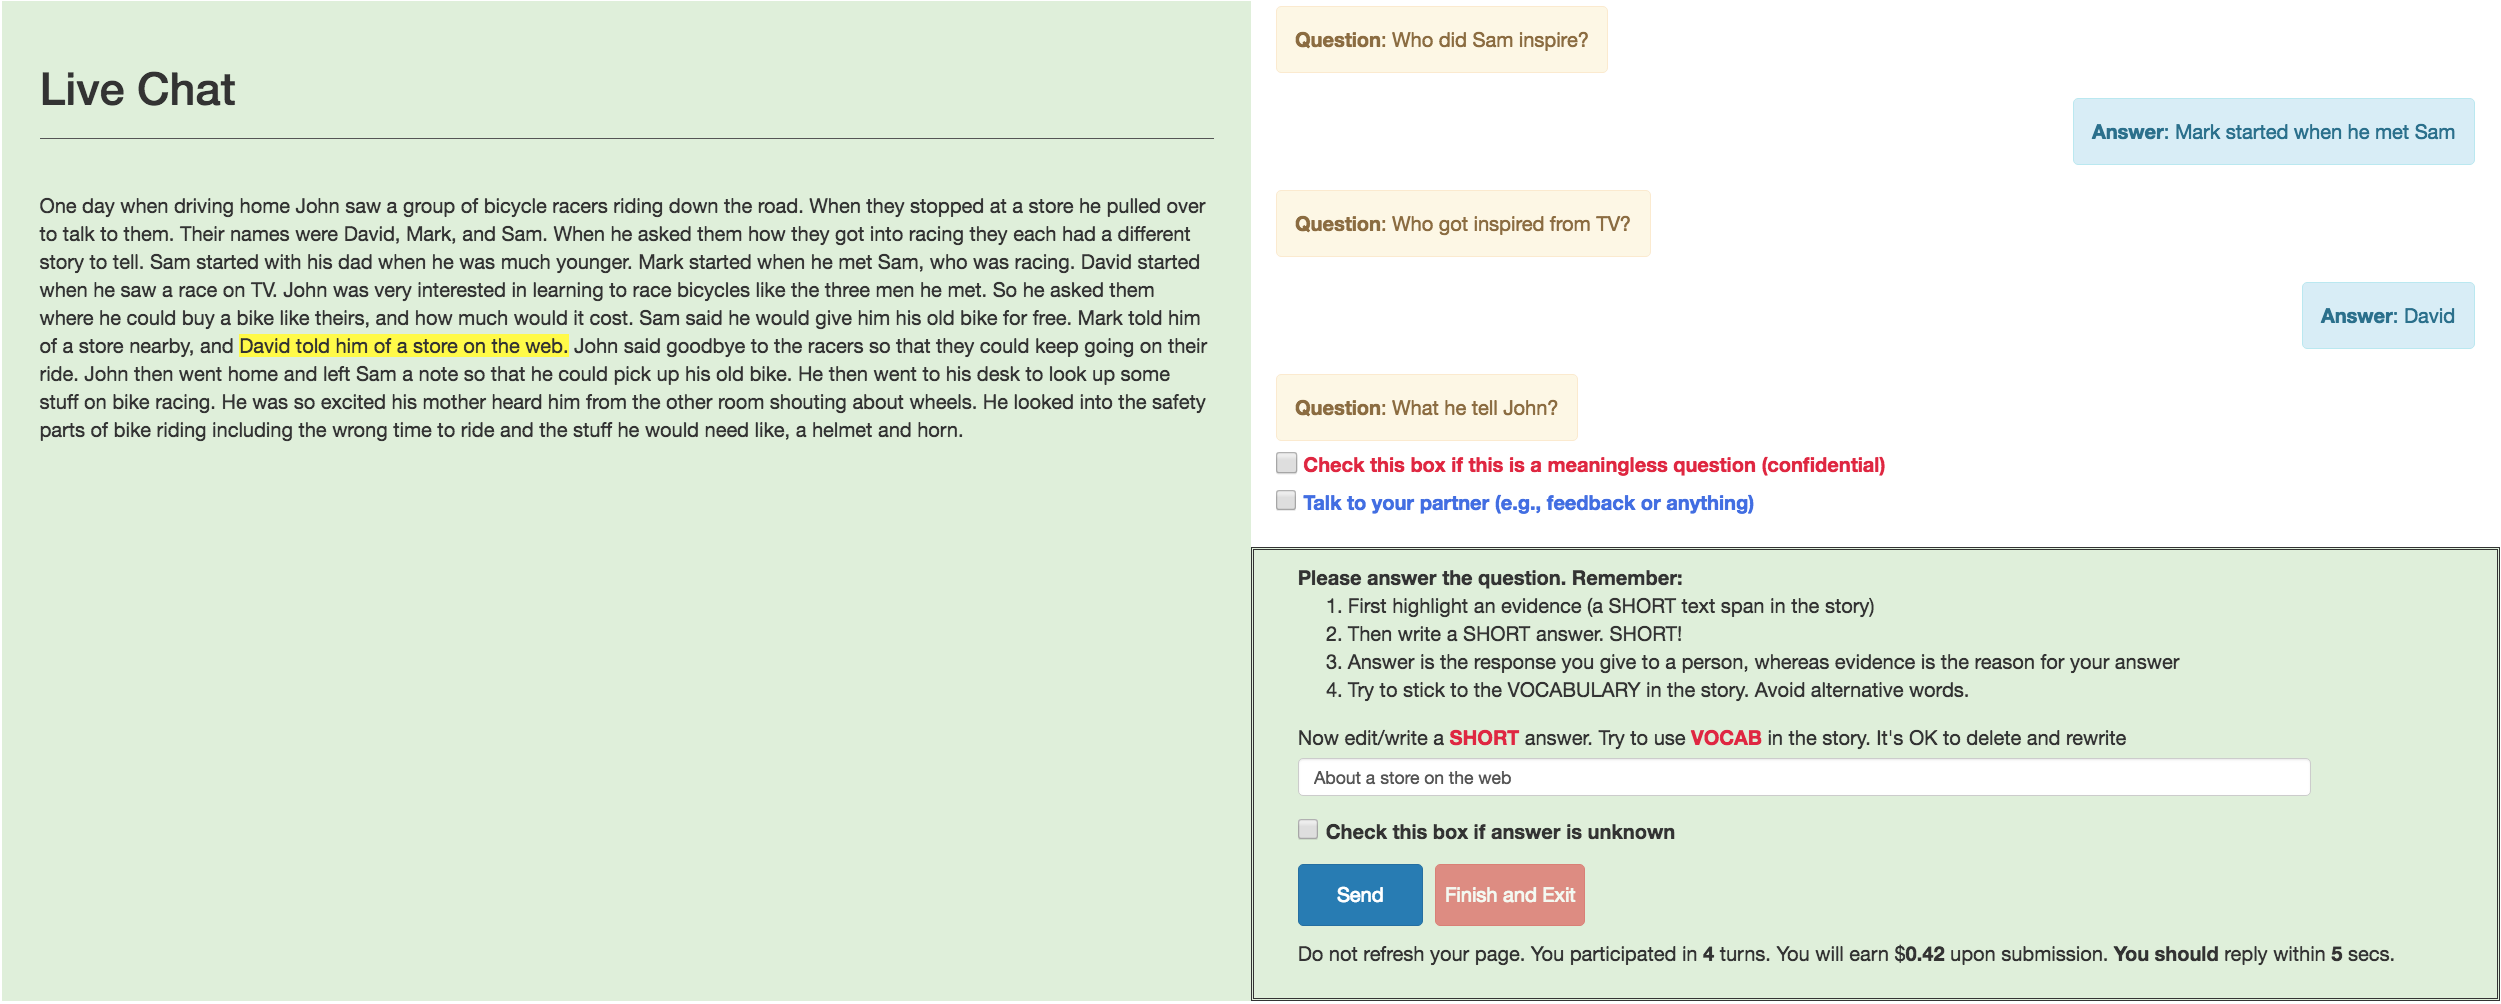
\includegraphics[scale=0.18]{img/coqa_answerer.png}
  \longcaption{The answerer interface of \sys{CoQA}}{\label{fig:coqa-answerer}The answerer interface of our \sys{CoQA} dataset.}
\end{figure}

We use the Amazon Mechanical Turk (AMT) to pair workers on a on a passage for which we use the ParlAI Mturk API \cite{miller2017parlai}. On average, each passage costs 3.6 USD for conversation collection and another 4.5 USD for collecting three additional answers for development and test data.


\paragraph{Collection interface.} We have different interfaces for a questioner and an answerer (Figure~\ref{fig:coqa-questioner} and Figure~\ref{fig:coqa-answerer}). A questioner's role is to ask questions, and an answerer's role is to answer questions in addition to highlighting rationales. We want questioners to avoid using exact words in the passage in order to increase lexical diversity. When they type a word that is already present in the passage, we alert them to paraphrase the question if possible. For the answers, we want answerers to stick to the vocabulary in the passage in order to limit the number of possible answers. We encourage this by automatically copying the highlighted text into the answer box and allowing them to edit copied text in order to generate a natural answer. We found 78\% of the answers have at least one edit such as changing a word's case or adding a punctuation.

\paragraph{Passage selection.} We select passages from seven diverse domains: children's stories from MCTest \cite{richardson2013mctest}, literature from Project Gutenberg\footnote{Project Gutenberg \url{https://www.gutenberg.org}}, middle and high school English exams from RACE \cite{lai2017race}, news articles from CNN \cite{hermann2015teaching}, articles from Wikipedia, science articles from AI2 Science Questions \cite{welbl2017crowdsourcing} and Reddit articles from the Writing Prompts dataset \cite{fan2018hierarchical}.

Not all passages in these domains are equally good for generating interesting conversations.
A passage with just one entity often result in questions that entirely focus on that entity.
We select passages with multiple entities, events and pronominal references  using Stanford \sys{CoreNLP} \cite{manning2014stanford}. We truncate long articles to the first few paragraphs that result in around 200 words.

Table~\ref{tab:coqa-domains} shows the distribution of domains.
We reserve the Science and Reddit domains for out-of-domain evaluation. For each in-domain dataset, we split the data such that there are 100 passages in the development set, 100 passages in the test set, and the rest in the training set. In contrast, for each out-of-domain dataset, we just have 100 passages in the test set without any passages in the training or the development sets.

\begin{table}
\centering
\begin{tabular}{lrrrr}
\toprule
\tf{Domain} &  \tf{\# Passages} &  \tf{\# Q/A} & \tf{Passage}  &  \tf{\# Turns per} \\
 & & \tf{pairs} & \tf{length} & \tf{passage} \\
\midrule
Children's Stories  & 750 & 10.5k & 211 &  14.0 \\
Literature  & 1,815 & 25.5k & 284  & 15.6 \\
Mid/High School Exams & 1,911 & 28.6k & 306  & 15.0 \\
News & 1,902 & 28.7k & 268 &  15.1 \\
Wikipedia & 1,821 & 28.0k & 245  & 15.4 \\
\midrule
\multicolumn{5}{c}{Out of domain} \\
\midrule
Science & 100 & 1.5k & 251  & 15.3\\
Reddit & 100 & 1.7k & 361 & 16.6 \\
\midrule
Total & 8,399 & 127k  & 271 & 15.2 \\
\bottomrule
\end{tabular}
\longcaption{Distribution of domains in \sys{CoQA}.}{\label{tab:coqa-domains} Distribution of domains in \sys{CoQA}.}
\end{table}

\paragraph{Collecting multiple answers.} Some questions in \sys{CoQA} may have multiple valid answers. For example, another answer for Q$_4$ in Figure~\ref{fig:coqa-example2} is \ti{A Republican candidate}. In order to account for answer variations, we collect three additional answers for all questions in the development and test data. Since our data is conversational, questions influence answers which in turn influence the follow-up questions. In the previous example, if the original answer was \ti{A Republican Candidate}, then the following question \ti{Which party does he belong to?} would not have occurred in the first place. When we show questions from an existing conversation to new answerers, it is likely they will deviate from the original answers which makes the conversation incoherent. It is thus important to bring them to a common ground with the original answer.

We achieve this by turning the answer collection task into a game of predicting original answers.
First, we show a question to a new answerer, and when she answers it, we show the original answer and ask her to verify if her answer matches the original.
For the next question, we ask her to guess the original answer and verify again.
We repeat this process until the conversation is complete.
In our pilot experiment, the human F1 score increased by 5.4\% when we use this verification setup.


\subsection{Dataset Analysis}
\label{sec:coqa-data-analysis}

What makes the \sys{CoQA} dataset conversational compared to existing reading comprehension datasets like \sys{SQuAD}? How does the conversation flow from one turn to the other? What linguistic phenomena do the questions in \sys{CoQA} exhibit? We answer these questions below.

\paragraph{Comparison with \sys{SQuAD 2.0}.}

\begin{figure}[ht]
\begin{center}
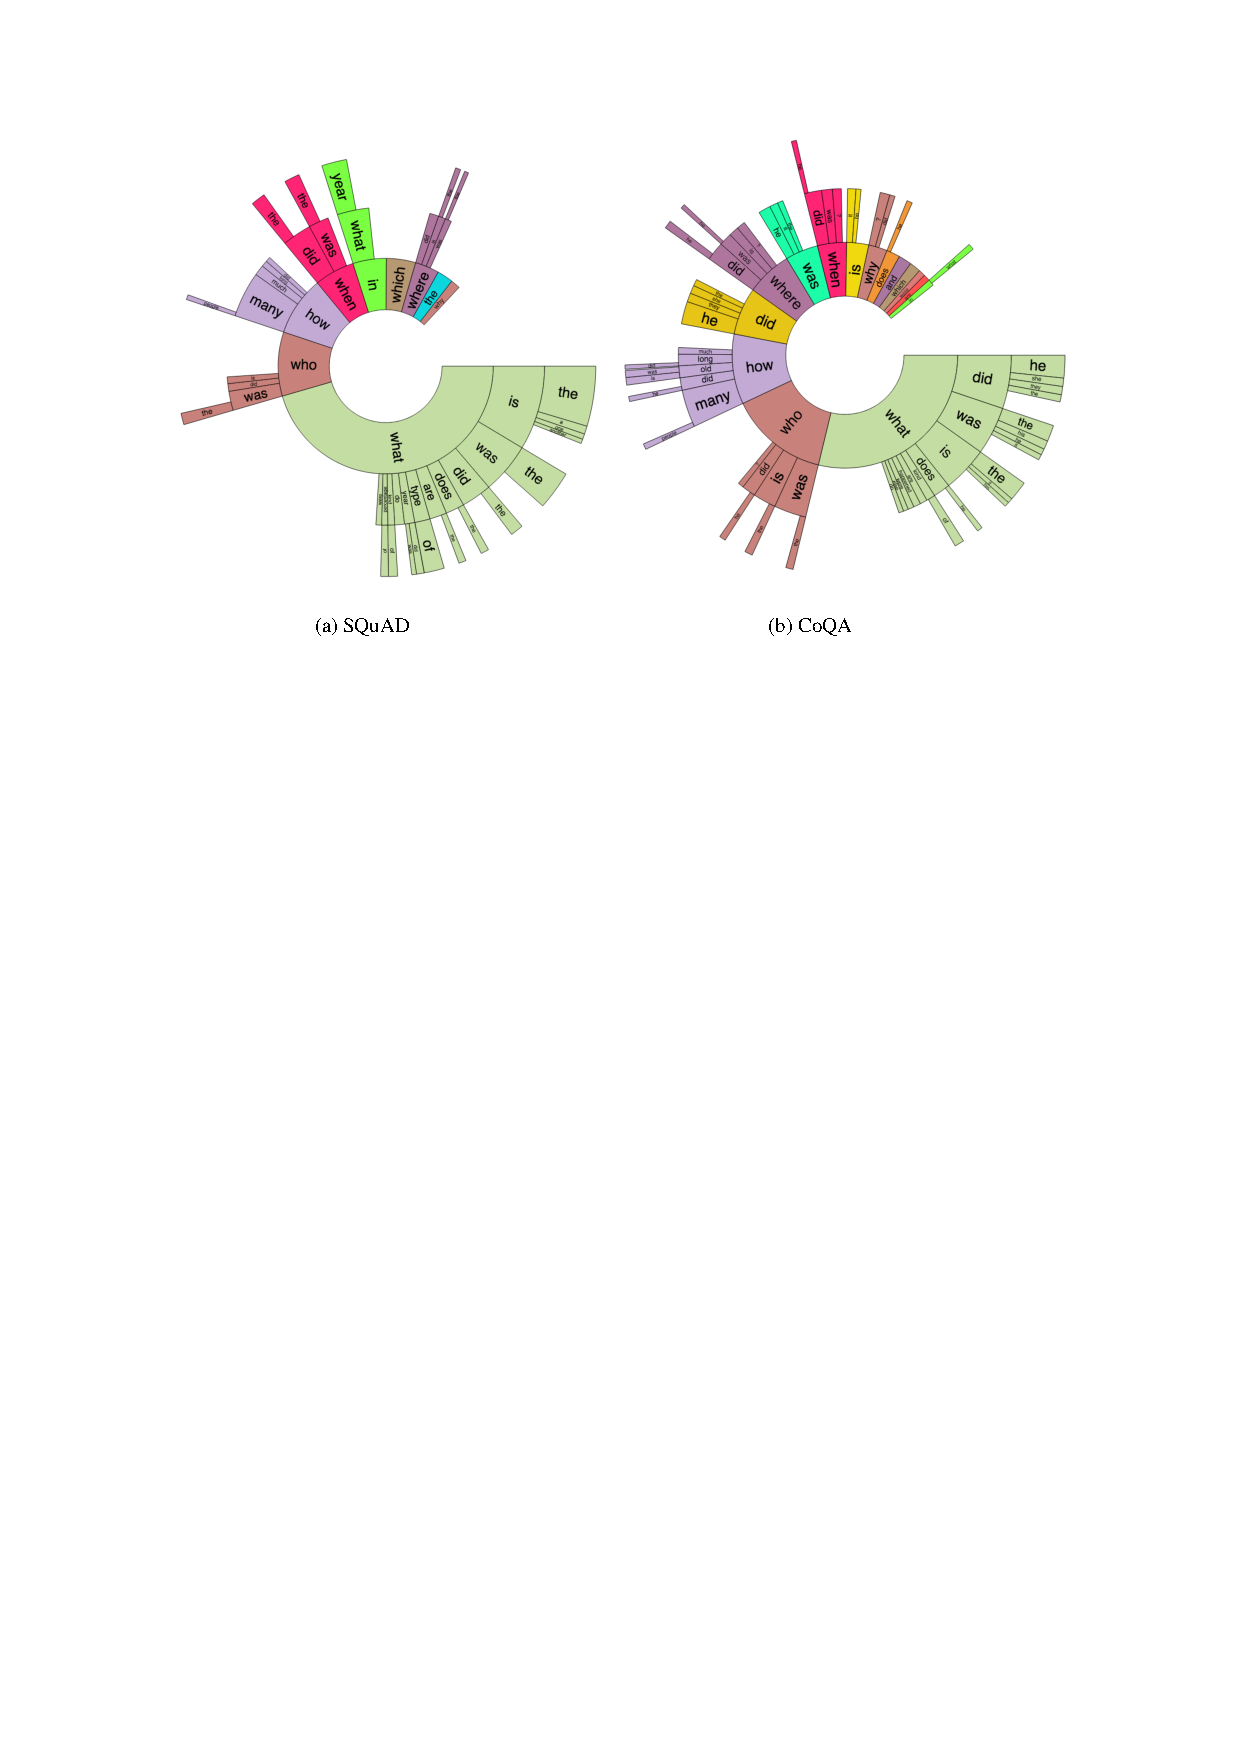
\includegraphics[height=8cm]{img/coqa_squad_comparison.pdf}
\end{center}
\longcaption{A comparison of questions in \sys{CoQA} and \sys{SQuAD 2.0} }{\label{fig:coqa-squad-comparison} Distribution of trigram prefixes of questions in \sys{SQuAD 2.0} and \sys{CoQA}.}
\end{figure}

In the following, we perform an in-depth comparison of \sys{CoQA} and \sys{SQuAD 2.0}~\cite{rajpurkar2018know}.  Figure~\ref{fig:coqa-squad-comparison} shows the distribution of frequent trigram prefixes. While coreferences are non-existent in \sys{SQuAD 2.0}, almost every sector of \sys{CoQA} contains coreferences (\ti{he, him, she, it, they})  indicating \sys{CoQA} is highly conversational. Because of the free-form nature of answers, we expect a richer variety of questions in \sys{CoQA} than \sys{SQuAD 2.0}.
While nearly half of \sys{SQuAD 2.0} questions are dominated by \ti{what} questions, the distribution of \sys{CoQA} is spread across multiple question types. Several sectors indicated by prefixes \ti{did, was, is, does, and} are frequent in \sys{CoQA} but are completely absent in \sys{SQuAD 2.0}.

Since a conversation is spread over multiple turns, we expect conversational questions and answers to be shorter than in a standalone interaction. In fact, questions in \sys{CoQA} can be made up of just one or two words (\ti{who?}, \ti{when?},  \ti{why?}).
As seen in Table~\ref{tab:squad-coqa-length}, on average, a question in \sys{CoQA} is only 5.5 words long while it is 10.1 for \sys{SQuAD}. The answers are also usually shorter in \sys{CoQA} than \sys{SQuAD 2.0}.

Table~\ref{tab:squad-coqa-answers} provides insights into the type of answers in \sys{SQuAD 2.0} and \sys{CoQA}.
While the original version of \sys{SQuAD 2.0}  \cite{rajpurkar2016squad} does not have any unanswerable questions, \sys{SQuAD 2.0} \cite{rajpurkar2018know} focuses solely on obtaining them resulting in higher frequency than in \sys{CoQA}. \sys{SQuAD 2.0} has 100\% extractive answers by design, whereas in \sys{CoQA}, 66.8\% answers can be classified as extractive after ignoring punctuation and case mismatches.\footnote{If punctuation and case are not ignored, only 37\% of the answers are extractive.}
This is higher than we anticipated. Our conjecture is that human factors such as wage may have influenced workers to ask questions that elicit faster responses by selecting text. It is worth noting that \sys{CoQA} has 11.1\% and 8.7\% questions with \ti{yes} or \ti{no} as answers whereas \sys{SQuAD 2.0} has 0\%. Both datasets have a high number of named entities and noun phrases as answers.



\begin{table}[h]
\centering
\begin{tabular}{p{3cm} r r}
\toprule
 & \bf \sys{SQuAD 2.0}  & \bf \sys{CoQA} \\
\midrule
Passage Length & 117 & 271 \\
Question Length & 10.1 & 5.5 \\
Answer  Length & 3.2 & 2.7 \\
\midrule
\end{tabular}
\longcaption{Data statistics in \sys{SQuAD 2.0} and \sys{CoQA}}{\label{tab:squad-coqa-length} Average number of words in passage, question and answer in \sys{SQuAD 2.0} and \sys{CoQA}.}
\end{table}

\begin{table}[h]
\centering
\begin{tabular}{p{3.5cm} r r}
\toprule
& \bf \sys{SQuAD 2.0}   & \bf \sys{CoQA}  \\
\midrule
Answerable & 66.7\% & 98.7\% \\
Unanswerable & 33.3\% & 1.3\% \\
\midrule
Extractive & 100.0\% & 66.8\% \\
Abstractive & 0.0\% & 33.2\% \\
\midrule
Named Entity & 35.9\% & 28.7\% \\
Noun Phrase & 25.0\% & 19.6\% \\
Yes & 0.0\% & 11.1\% \\
No & 0.1\% & 8.7\% \\
Number & 16.5\% & 9.8\% \\
Date/Time & 7.1\% & 3.9\% \\
Other & 15.5\% & 18.1\% \\
\bottomrule
\end{tabular}
\longcaption{Distribution of answer types in \sys{SQuAD 2.0} and \sys{CoQA}}{\label{tab:squad-coqa-answers} Distribution of answer types in \sys{SQuAD 2.0} and \sys{CoQA}.}
\end{table}

\paragraph{Conversation flow.}
A coherent conversation must have smooth transitions between turns.
We expect the narrative structure of the passage to influence our conversation flow.
We split the passage into 10 uniform chunks, and identify chunks of interest of a given turn and its transition based on rationale spans.

\begin{figure}[!t]
\begin{center}
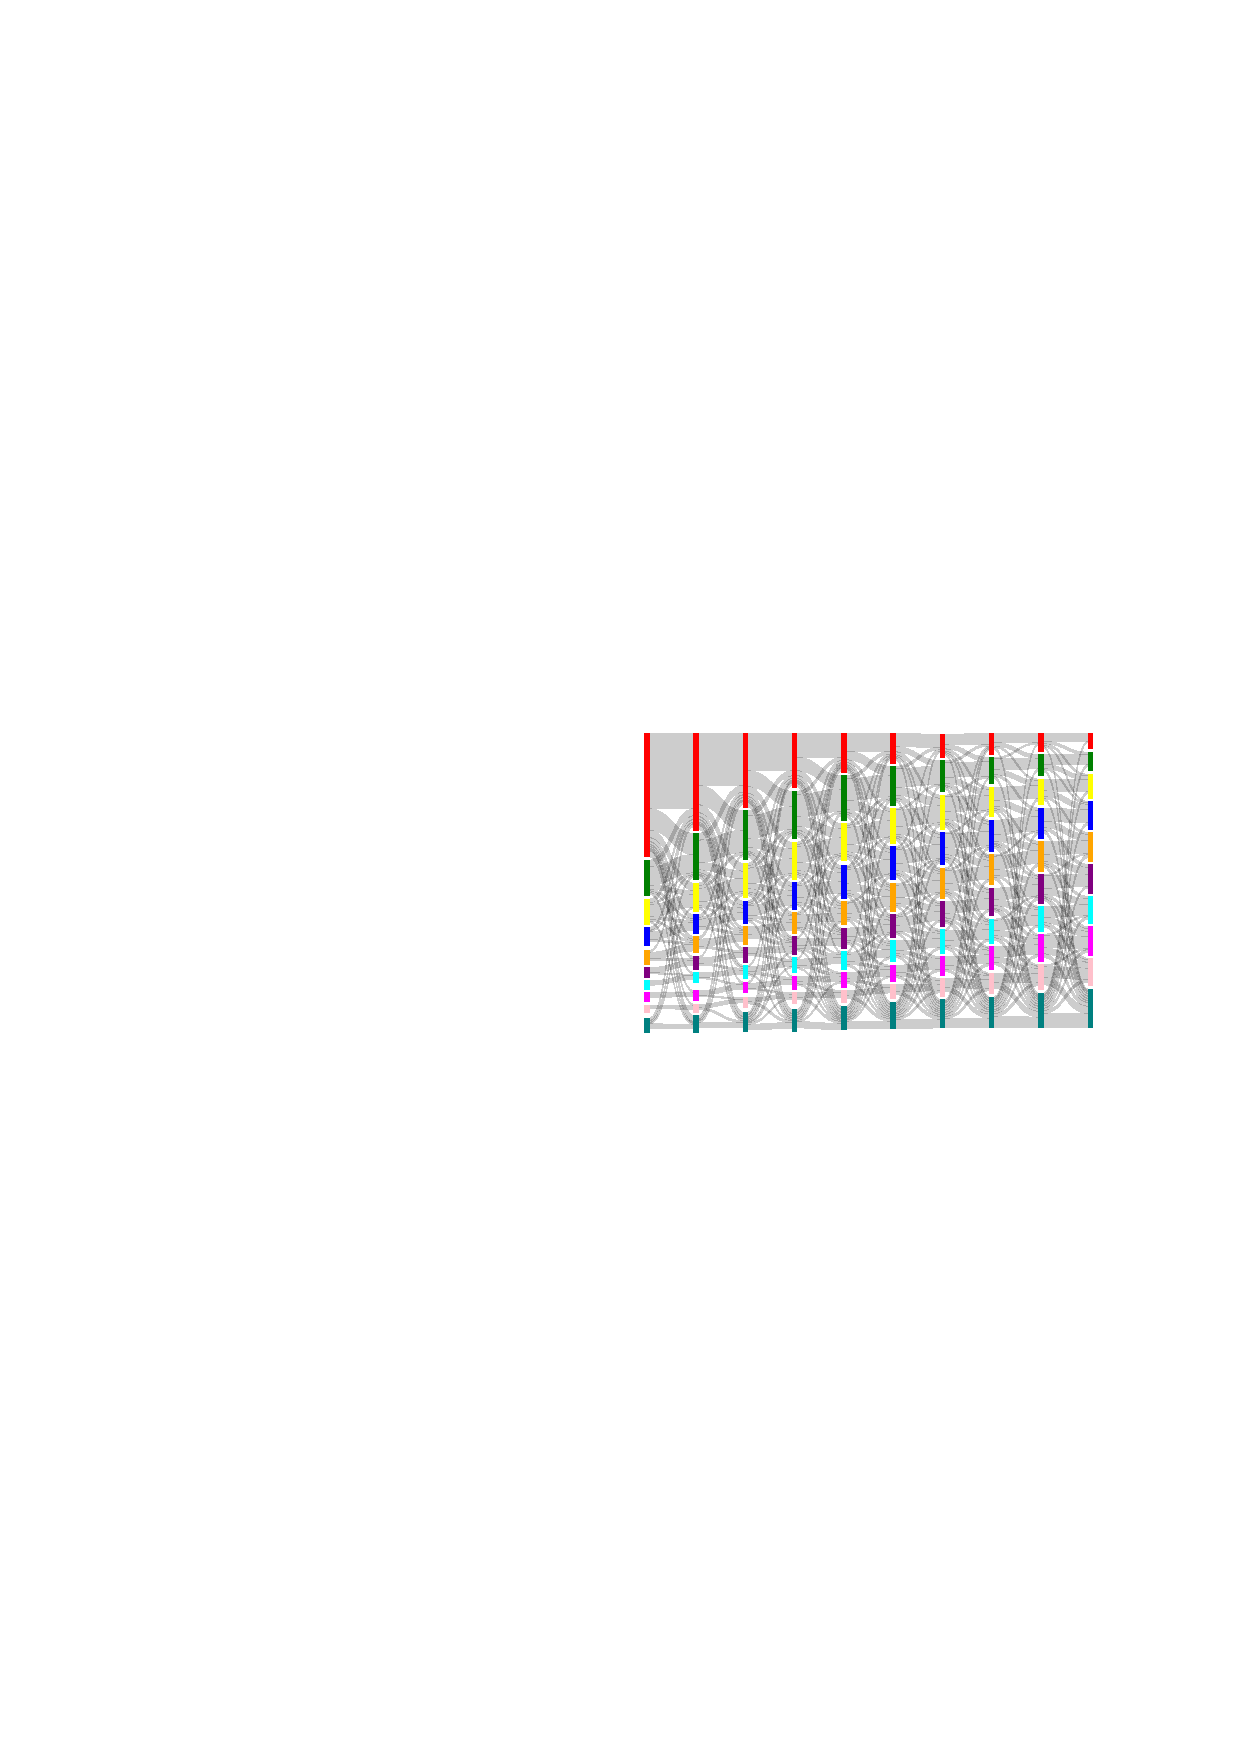
\includegraphics[height=9cm]{img/coqa_conversation_flow.pdf}
\end{center}
\longcaption{Conversation Flow in \sys{CoQA}}{\label{fig:coqa-conversation-flow} Chunks of interests as a conversation progresses. The x-axis indicates the turn number and
the y-axis indicates the passage chunk containing the rationale. The height of a chunk indicates the concentration of conversation in that chunk. The width of the bands is proportional to the frequency of transition between chunks from one turn to the other.}
\end{figure}


Figure~\ref{fig:coqa-conversation-flow} portrays the conversation flow of the top 10 turns.
The starting turns tend to focus on the first few chunks and as the conversation advances, the focus shifts to the later chunks. Moreover, the turn transitions are smooth, with the focus often remaining in the same chunk or moving to a neighbouring chunk. Most frequent transitions happen to the first and the last chunks, and likewise these chunks have diverse outward transitions.

\paragraph{Linguistic phenomena.}

\begin{table}[!t]
\centering
\small
\begin{tabular}{lp{7cm}c}
\toprule
\bf Phenomenon & \bf Example & \bf Percentage \\
\midrule
\multicolumn{3}{c}{Relationship between a question and its passage} \\
\midrule
Lexical match & Q: Who had to rescue her?& 29.8\% \\
& A: the coast guard \\
& R: Outen was rescued by the coast guard \\
Paraphrasing & Q: Did the wild dog approach? & 43.0\% \\
& A: Yes \\
& R: he drew cautiously closer \\
Pragmatics &  Q:               Is Joey a male or female?  &  27.2\% \\
 & A:  Male \\
& R: it looked like a stick man so she kept \textbf{him}. She named her new noodle friend Joey \\
\midrule
\multicolumn{3}{c}{Relationship between a question and its conversation history} \\
\midrule
No coreference & Q: What is IFL? & 30.5\% \\
Explicit coreference & Q: Who had Bashti forgotten? & 49.7\% \\
& A: the puppy \\
& Q: What was \textbf{his} name? \\
Implicit coreference & Q: When will Sirisena be sworn in? & 19.8\% \\
& A: 6 p.m local time  \\
& Q: \textbf{Where}?\\
\bottomrule
\end{tabular}
\longcaption{Linguistic phenomena in \sys{CoQA} questions}{\label{tab:ling-phenomena}Linguistic phenomena in \sys{CoQA} questions.}
\end{table}
We further analyze the questions for their relationship with the passages and the conversation history. We sample 150 questions in the development set and annotate various phenomena as shown in Table~\ref{tab:ling-phenomena}.

If a question contains at least one content word that appears in the passage, we classify it as \ti{lexical match}. These comprise around 29.8\% of the questions. If it has no lexical match but is a paraphrase of the rationale, we classify it as \ti{paraphrasing}. These questions contain phenomena such as synonymy, antonymy, hypernymy, hyponymy and negation.
These constitute a large portion of questions, around 43.0\%. The rest, 27.2\%, have no lexical cues, and we classify them under \ti{pragmatics}. These include phenomena like common sense and presupposition. For example, the question \ti{Was he loud and boisterous?} is not a direct paraphrase of the rationale \ti{he dropped his feet with the lithe softness of a cat} but the rationale combined with world knowledge can answer this question.

For the relationship between a question and its conversation history, we classify questions into whether they are dependent or independent on the conversation history. If dependent, whether the questions contain an explicit marker or not.

As a result, around 30.5\% questions do not rely on coreference with the conversational history and are answerable on their own. Almost half of the questions (49.7\%) contain explicit coreference markers such as \ti{he, she, it}. These either refer to an entity or an event introduced in the conversation.
The remaining 19.8\% do not have explicit coreference markers but refer to an entity or event implicitly.
